\documentclass{article}
\usepackage[UTF8]{ctex}
% Replace `letterpaper' with`a4paper' for UK/EU standard size
\usepackage[a4paper,top=2cm,bottom=2cm,left=3cm,right=3cm,marginparwidth=1.75cm]{geometry}

% Useful packages
\usepackage{amsmath}
\usepackage{graphicx}
\usepackage[colorlinks=true, allcolors=blue]{hyperref}
\usepackage{graphicx} %插入图片的宏包
\usepackage{float} %设置图片浮动位置的宏包
\usepackage{subfigure} %插入多图时用子图显示的宏包
\usepackage{parskip}
\usepackage{indentfirst} 
\setlength{\parindent}{2em}
\usepackage{hyperref}  
\usepackage{tikz}
\allowdisplaybreaks
\usepackage{multirow}
\usepackage{amsmath}
\usepackage{amsfonts,amssymb} 
\usepackage{xcolor} % 用于显示颜色
\usepackage{listings} % 用于插入代码
\lstset{
	basicstyle          =   \sffamily,          % 基本代码风格
	keywordstyle        =   \bfseries,          % 关键字风格
	commentstyle        =   \rmfamily\itshape,  % 注释的风格,斜体
	stringstyle         =   \ttfamily,  % 字符串风格
	flexiblecolumns,                % 别问为什么,加上这个
	numbers             =   left,   % 行号的位置在左边
	showspaces          =   false,  % 是否显示空格,显示了有点乱,所以不现实了
	numberstyle         =   \zihao{-5}\ttfamily,    % 行号的样式,小五号,tt等宽字体
	showstringspaces    =   false,
	captionpos          =   t,      % 这段代码的名字所呈现的位置,t指的是top上面
	frame               =   lrtb,   % 显示边框
}

\lstdefinestyle{R}{
	language        =   R, % 语言选Python
	basicstyle      =   \zihao{-5}\ttfamily,
	numberstyle     =   \zihao{-5}\ttfamily,
	keywordstyle    =   \color{blue},
	keywordstyle    =   [2] \color{teal},
	stringstyle     =   \color{magenta},
	commentstyle    =   \color{red}\ttfamily,
	breaklines      =   true,   % 自动换行,建议不要写太长的行
	columns         =   fixed,  % 如果不加这一句,字间距就不固定,很丑,必须加
	basewidth       =   0.5em,
}

\title{The first Homework of Statistical Computing}
\author{Lin Zikai}

\begin{document}
	\maketitle
    \tableofcontents

\section{Exercise 3.5}
    \subsection{R code}
        \lstinputlisting[style = R,
        caption={R code of Exercise 3.5},
        label = {3.5_R_code}
        ]{hw1_3.5.R}
    \subsection{experiment result}
        I have repeated the experiment for 5 times. Compared with the theoretical probability,
        the five relative frequency tables are as follows:
        
        \begin{table}[H]
            \centering
            \caption{experiment results of Exercise 3.5}
            \begin{tabular}{llllll}
            \hline
                             & 0      & 1      & 2      & 3      & 4      \\ \hline
            theoretical prob & 0.1000 & 0.2000 & 0.2000 & 0.2000 & 0.3000 \\
            empirical prob 1 & 0.1100 & 0.2275 & 0.1875 & 0.2025 & 0.2725 \\
            empirical prob 2 & 0.1200 & 0.2125 & 0.1900 & 0.1825 & 0.2950 \\
            empirical prob 3 & 0.1375 & 0.1925 & 0.1650 & 0.2125 & 0.2925 \\
            empirical prob 4 & 0.1200 & 0.1950 & 0.1825 & 0.2025 & 0.3000 \\
            empirical prob 5 & 0.1075 & 0.2275 & 0.2250 & 0.1725 & 0.2675 \\ \hline
            \end{tabular}
            \end{table}

\section{Exercise 3.6}
    Suppose Y is a random variable generated from density function $g(y)$, 
    and U from Uniform$(0,1)$. According to the procedure of the Acceptance-Rejection method, 
    we have
    \begin{align*}
        &P(\text{accepted}|Y=y) = P(U<\frac{f(y)}{cg(y)}|Y=y) = \frac{f(y)}{cg(y)} \\
        &P(\text{Y is accepted for one iteration}) \\
        & = \int_{-\infty}^{+\infty}P(\text{accepted}|Y=y)g(y)\,\text{d}y \\
         &= \int_{-\infty}^{+\infty}\frac{f(y)}{cg(y)}g(y)\,\text{d}y \\
        & = \frac{1}{c} \int_{-\infty}^{+\infty}f(y) \\
        & = \frac{1}{c}
    \end{align*}
    And finally we have
    \begin{align*}
        f_{Y|accepted}(y) 
        &= \frac{f(Y=y \enspace \text{and} \enspace \text{accpeted})}{P(\text{Y is accepted for one iteration})} \\
        &= \frac{P(\text{accepted}|Y=y)g(y)}{P(\text{Y is accepted for one iteration})} \\
        &= \frac{\frac{f(y)}{cg(y)}g(y)}{\frac{1}{c}} \\
        &= f(y)
    \end{align*}

\section{Exercise 3.9}
    \subsection{R code}
        \lstinputlisting[style = R,
        caption={R code of Exercise 3.9},
        label = {3.9_R_code}
        ]{hw1_3.9.R}
    \subsection{histogram density estimate}
        The histogram (orange bars) density estimate by 10000 samples is as follows:
        \begin{figure}[H]
            \centering  %图片全局居中
            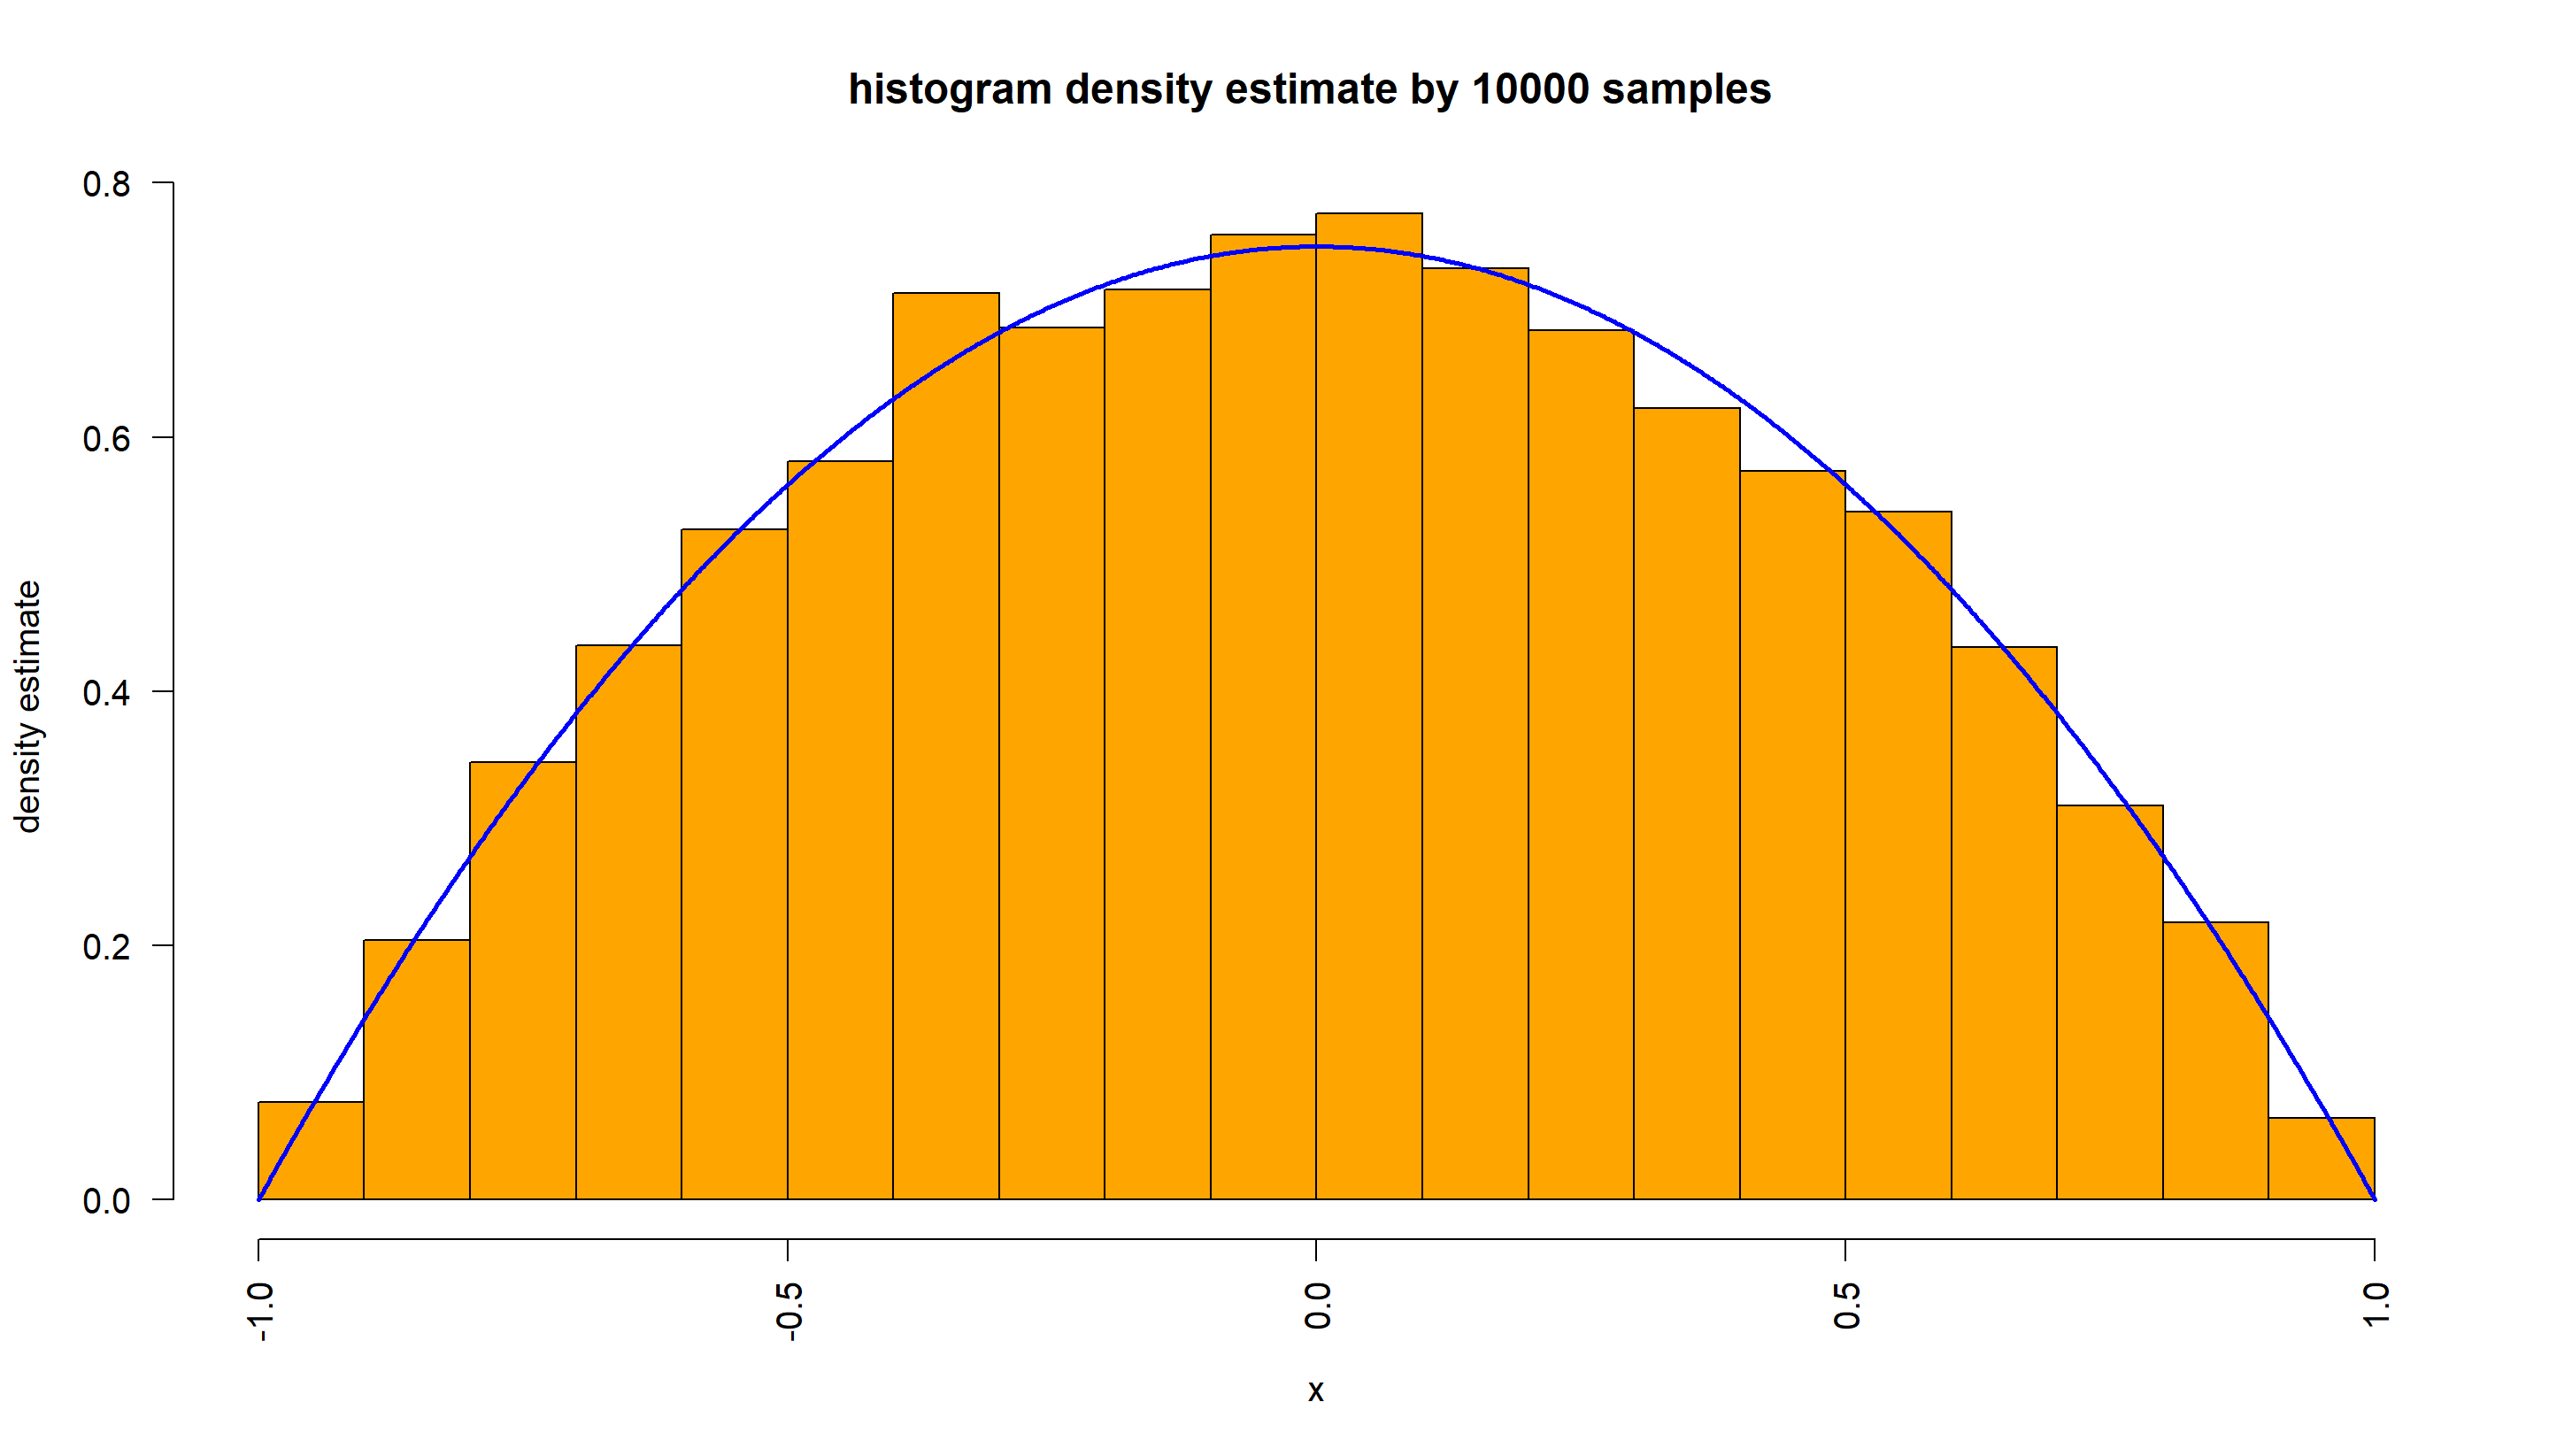
\includegraphics[width=0.8\textwidth]{3.9 estimate_of_fe.png}
            \caption{histogram density estimate of $f_e$}
        \end{figure}
        The blue line is $f_e$ density function, which is consistent with the histogram.

\section{Exercise 3.10}
    Assume that the variates generated by the algorithm in Exercise 3.9 is from
     a density $f(x)$. From the Law of Total probability, we have
     \begin{align*}
        f(x) &= f_{U_3}(x\bigg||U_3|\text{ is not maximum}) P(|U_3|\text{ is not maximum})
            + f_{U_2}(x\bigg||U_3| \text{ is maxium}) P(|U_3|\text{ is maximum}) \\
            & = f_{U_3}(x) P(|U_3|\text{ is not maximum}\bigg|U_3=x)
            + f_{U_2}(x) P(|U_3|\text{ is maximum}\bigg| U_2=x) \\
            & = \frac{1}{2} [1-P(|U_3|\text{ is maximum}\bigg|U_3=x)] 
            + \frac{1}{2} P(|U_3|\text{ is maximum}\bigg|U_2=x) \\
            & = \frac{1}{2} [1-P(|U_1|<|x|, |U_2|<|x| \bigg|U_3=x)] 
            + \frac{1}{2} P(|U_3|>|U_1|\bigg| U_2=x,|U_3|>|x|) P(|U_3|>|x|\bigg| U_2=x) \\
            &= \frac{1}{2}(1-x^2) + \frac{1}{2} \frac{\int_{|x|}^1t\,\text{d}t}{(1-|x|)}(1-|x|) \\
            &= \frac{3}{4}(1-x^2)
     \end{align*} 
     
     Therefore, the algorithm given in Exercise 3.9 generates variates from the density $f_e$.
     
\section{Exercise 3.12 and 3.13}
	\subsection{R code}
	\lstinputlisting[style = R,
	caption={R code of Exercise 3.12 and 3.13},
	label = {3.12_R_code}
	]{hw1_3.12+3.13.R}
	\subsection{density histogram}
	 The empirical and theoretical (Pareto) distributions are as follows:
	 \begin{figure}[H]
	 	\centering  %图片全局居中
	 	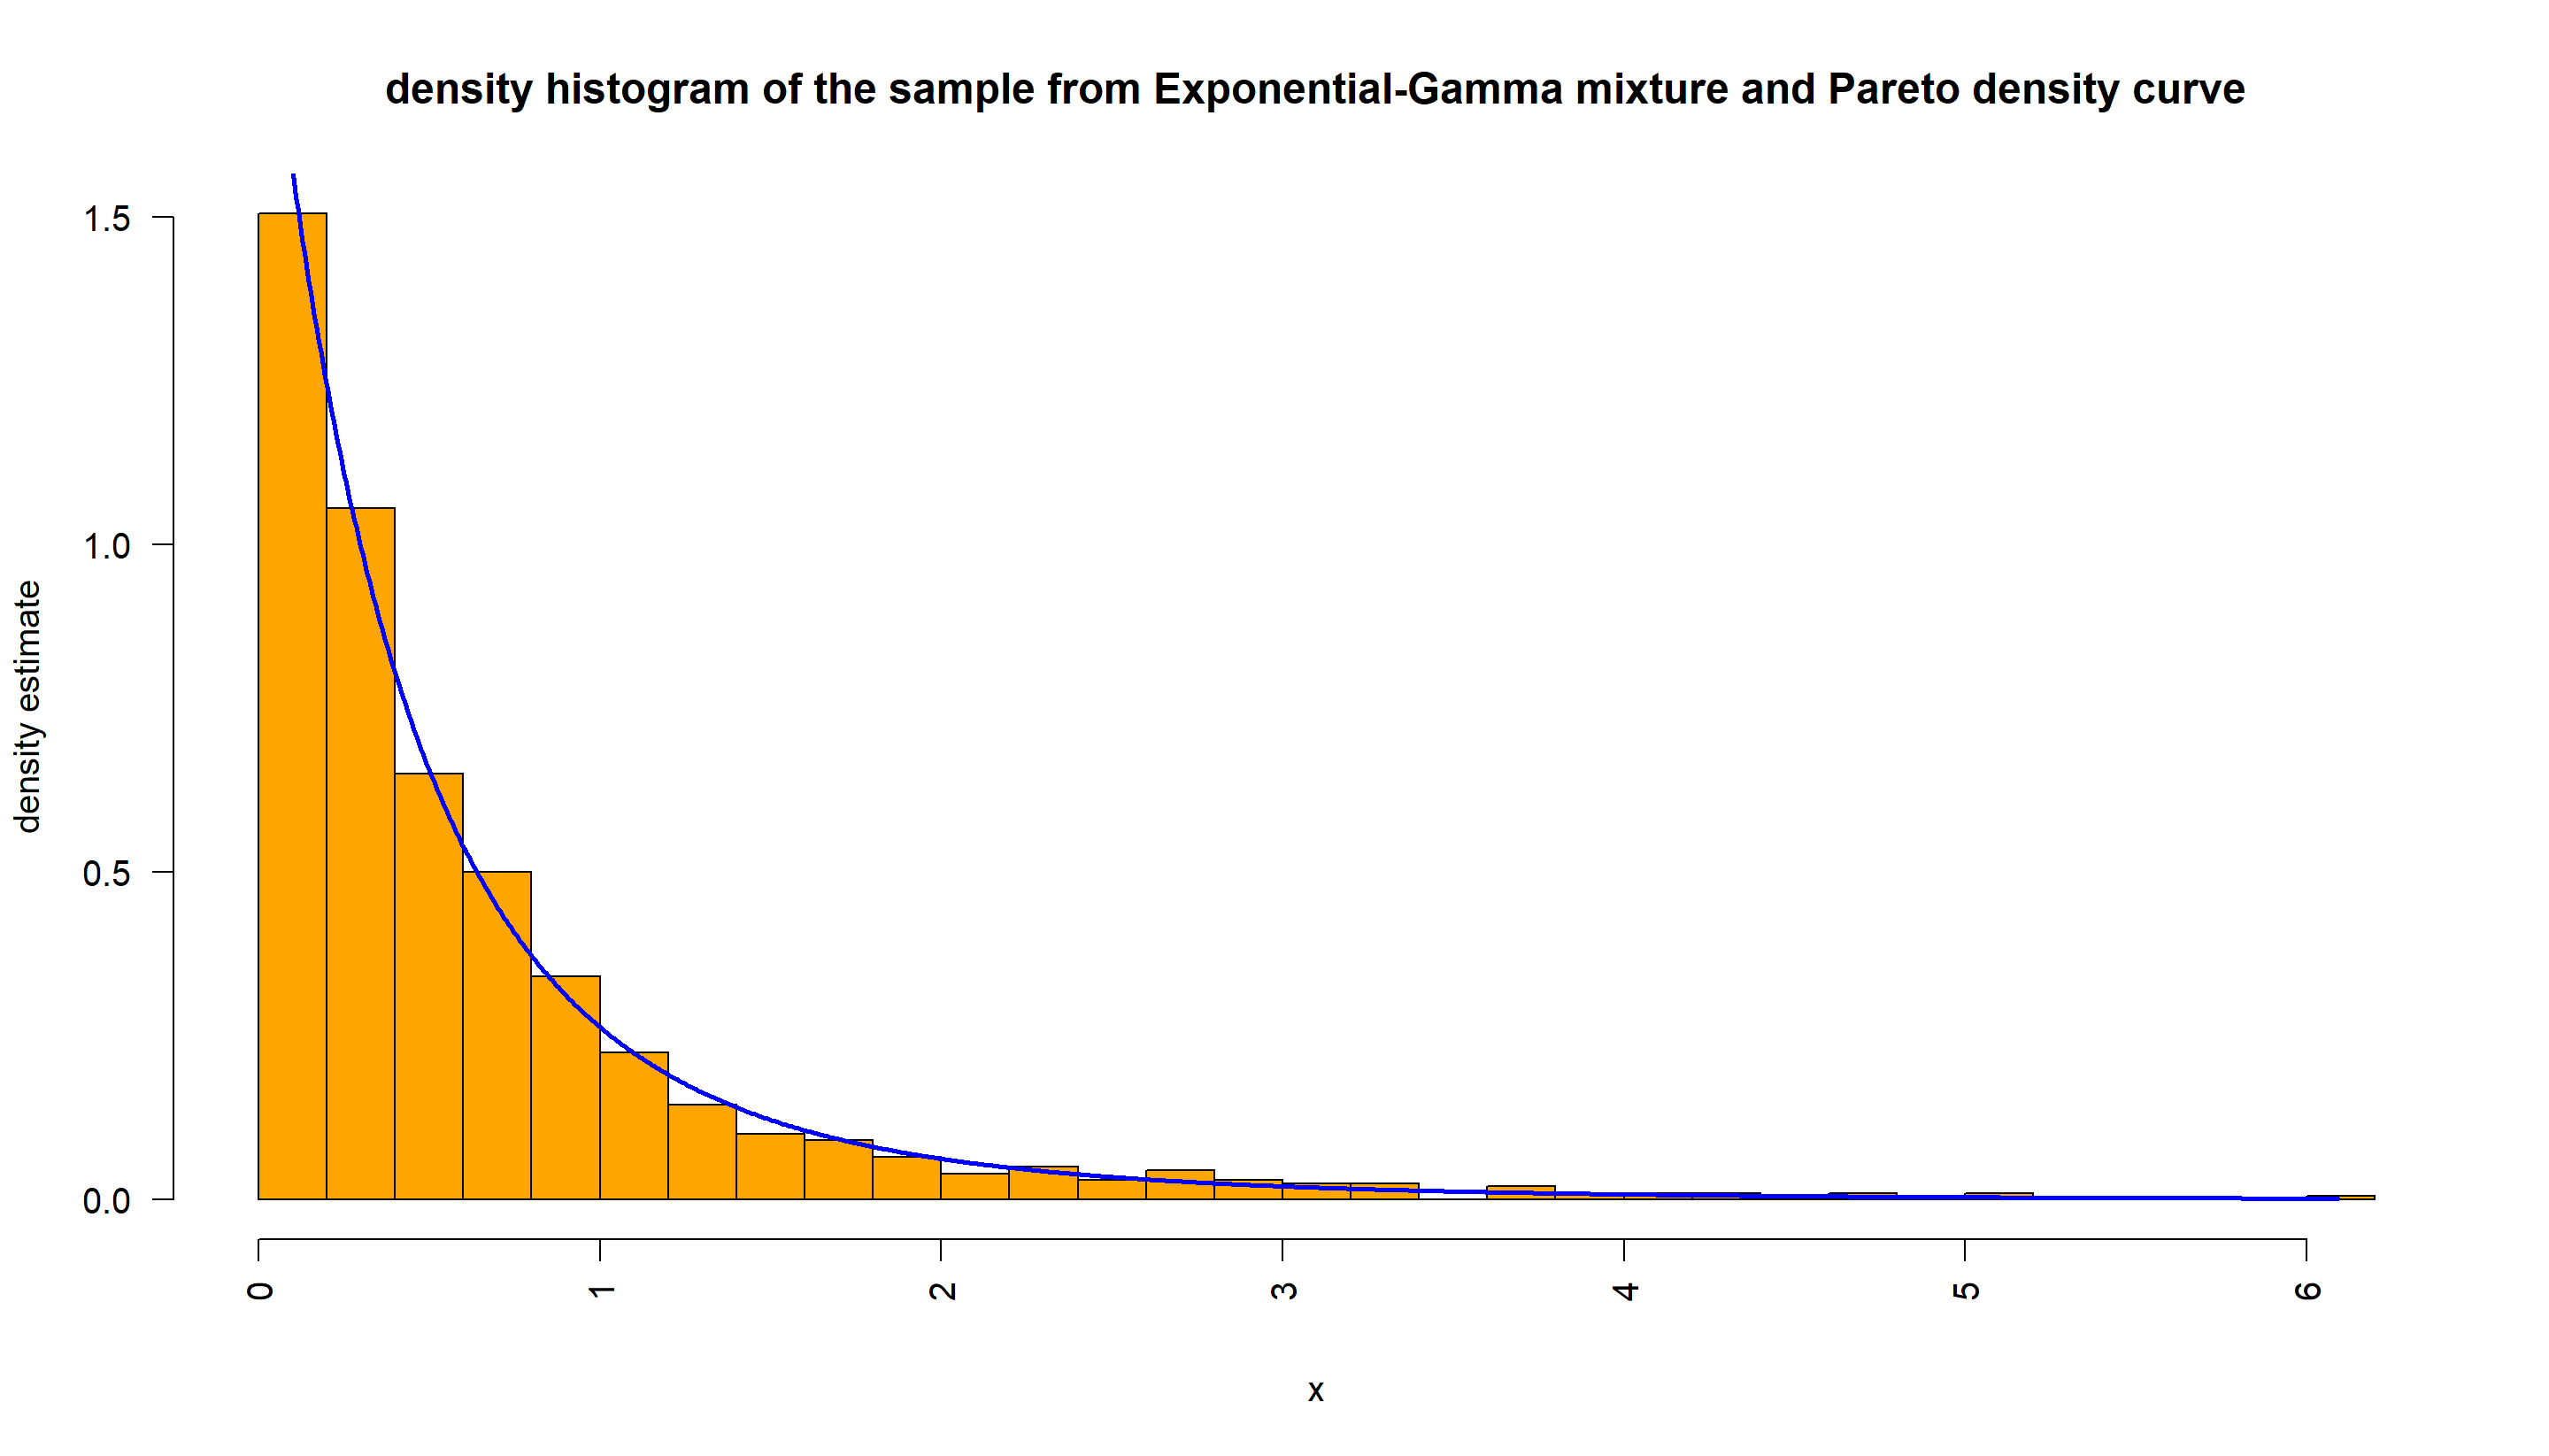
\includegraphics[width=0.8\textwidth]{Exp-Gamma mixture}
	 	\caption{Histogram of sample from Exp-Gamma mixture and the Pareto density Curve}
	 \end{figure}
	 
	 We can observe that the density histogram of the sample from Exponential-Gamma mixture is consistent with the Pareto density curve.
	 
\section{Exercise 3.14}
    \subsection{R code}
        \lstinputlisting[style = R,
         caption={R code of Exercise 3.14},
         label = {3.14_R_code}
         ]{hw1_3.14.R}
    \subsection{scatter plots for each pair of variables}
    \begin{figure}[H]
        \centering  %图片全局居中
        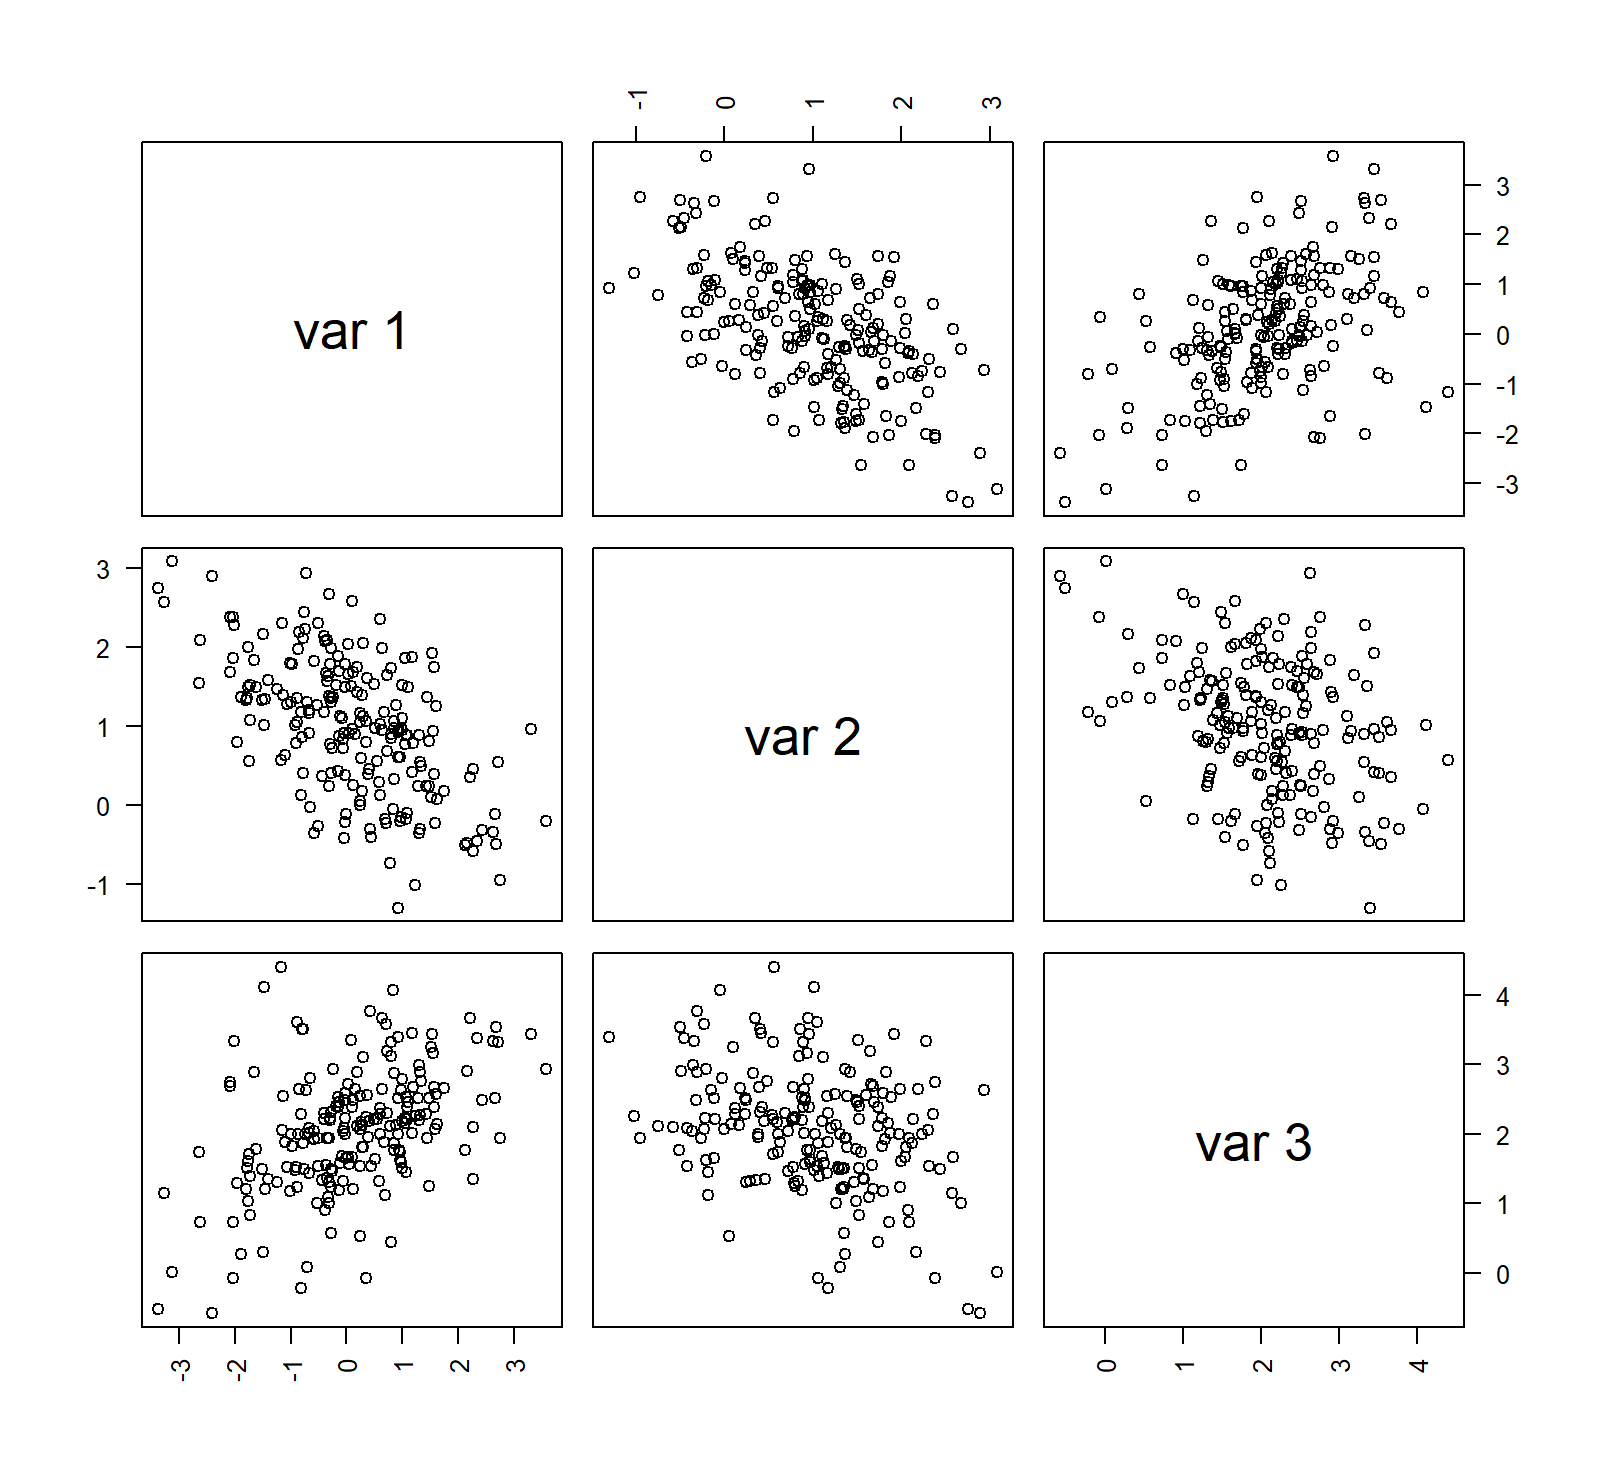
\includegraphics[width=0.8\textwidth]{pairs}
        \caption{scatter plots for each pair of variables}
        \label{pairPlot}
    \end{figure}
    
    From fig\ref{pairPlot}, we can see that the scatter plot of var1 and var2 (Plot-12 for short) is centered at
    approximately (0,1), scatter plot of var1 and var3 (Plot-13 for short) is centered at approximately (0,2),
    and scatter plot of var2 and var3 (Plot-23 for short) is centered at (1,2), which correspond to the parameters
    $\mu = (0,1,2)$. On the other hand,  Plot-12 and Plot-23 are distributed around the main
    diagonal, while Plot-13 is distributed around the secondary diagonal, which are consistent with the parameters
    $\rho_{12}=\rho_{23}=-0.5, \, \rho_{13} = 0.5$.
\end{document}